\begin{mainbar}
    \textbf{Homero Javier Velasteguí Izurieta}
\end{mainbar}

\columnratio{0.5}
\setlength{\columnsep}{0.75cm}
\setlength{\columnseprule}{3pt}
\colseprulecolor{lightcol}



\begin{paracol}{2}
\begin{leftcolumn}


\begin{wrapfigure}{l}{0.18\textwidth}
  \begin{center}
    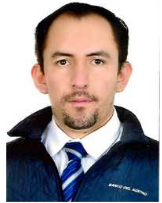
\includegraphics[width=0.2\textwidth]{Portada/Foto.png}  
  \end{center}
\end{wrapfigure}
Soy un idealista con una pasión innata por las investigaciones científicas y un enfoque especializado en el desarrollo de sistemas embebidos y la seguridad tecnológica.\\ Mi experiencia como Docente Coordinador del área académica de Industria Tecnología y Comunicación en la Pontificia Universidad Católica del Ecuador Sede Esmeraldas respalda mi sólida formación como Ingeniero en Electrónica y Comunicaciones, así como mi título de Magister en Ciberseguridad.\\
Mi visión de superación personal y profesional me impulsa constantemente a buscar nuevas oportunidades para adquirir conocimientos y aplicarlos de manera innovadora. Mi objetivo es seguir contribuyendo al progreso tecnológico y la protección de la información en el mundo digital, colaborando en equipos multidisciplinarios y enfrentando nuevos desafíos con entusiasmo.

\end{leftcolumn}

\begin{rightcolumn} 



\pvsection{Educación}

\begin{dport}
    \pvevent
	{Magister en Ciberseguridad}
	{Pontificia Universidad Católica del Ecuador }
	{Artículo IEEE Xplore:“IoT-based Security Alarm Protocol”}
	{}
	{\textbf{2020 - 2021}}
\end{dport}


\begin{lport}
    \pvevent
	{Ingeniería en Electrónica y Comunicaciones}
	{Universidad Técnica de Ambato }
	{Tesis:“Enabling Electronic System for Emergency Alerts”}
	{}
	{\textbf{2020 - 2021}}
\end{lport}

\end{rightcolumn}
\end{paracol}
\setlength{\parindent}{0pt}
\textcolor{lightcol}{ \rule{1.02\textwidth}{3pt} }

